\section{Structured Assurance Case Metamodel}
\label{sec:sacm}
The \textit{Structured Assurance Case Metamodel} (SACM) is standardised by the Object Management Group (OMG). The intention of the metamodel is to promote model-based approach in the process of \textit{System Assurance}, which is currently a manual approach that produces artefacts (i.e. Assurance Cases) that are not consumable by computers. SACM is created to support structural argumentation approaches such as the \textit{Goal Structuring Notation} (GSN) and \textit{Claims, Arguments and Evidence} (CAE). 

SACM captures not only fundamental concepts in the process of \textit{System Assurance} such as \textit{Claim}s and the relationships between \textit{Claim}s, it also captures concepts such as \textit{Artifact}s and \textit{Terminologi}es, in the sense that supporting evidence and information involved in the argument can be modelled in greater precision. In addition, SACM promotes \textit{modularity}, in the sense that assurance cases are organised in packages, which in turn organise argumentations, evidence and terminologies in corresponding packages. SACM also promotes \textit{openness} in the sense that external information (such as external models and/or documents) can be linked via the facilities provided. 

In this section, we provide a definitive guide to SACM. We discuss the packages in SACM and their intended usage. 
We will provide two types of examples to demonstrate how SACM can be used: for simple concepts to explain without further context we will use in-place examples; and for complex concepts which requires the context of understanding the entirety of SACM we will use dedicated examples, provided at the end of this section.
Since OMG has not standardised the concrete syntax of SACM, we will use object diagrams in the examples. 

\subsection{SACM Overview}
In overview, SACM is organised in five packages, as illustrated in Figure \ref{fig:overview}. The \textit{Base} package provides the foundation of SACM, which will be discussed in Section \ref{sec:basePack}. The \textit{Argumentation} package captures the concepts used in arguing system properties (such as safety and/or security)\footnote{System properties refer to the safety and/or security in the context of this paper, hereafter.}, which will be discussed in Section \ref{sec:argPack}. The \textit{Terminology} package captures the concepts used in expressing the arguments regarding system properties, which will be discussed in Section \ref{sec:termPack}. The \textit{Artifact} package captures the concepts used in providing evidence for the arguments made for system properties. The \textit{Artifact} package will be discussed in Section \ref{sec:artiPack}. Finally, the \textit{AssuranceCase} package captures the concepts in \textit{System Assurance}, which combines all the elements in other SACM packages to form a \textit{System Assurance Case}. The \textit{AssuranceCase} package will be discussed in Section \ref{sec:acPack}.

\begin{figure}
	\centering
	
	
	
	
	
	
	
	
	
	
	
	
	
	
	
	
	
	
	
	
	
	
	
	
	
	
	
	
	
	
	
	
	
	
	
	
	
	
	
	
	
	
	
	
	
	
	
	
	
	
	
	
	
	
	
	
	
	
	
	
	
	
	
	
	
	
	
	
	
	
	
	
	
	
	
	
	
	
	
	
	
	
	
	
	
	
	
	
	
	
	
	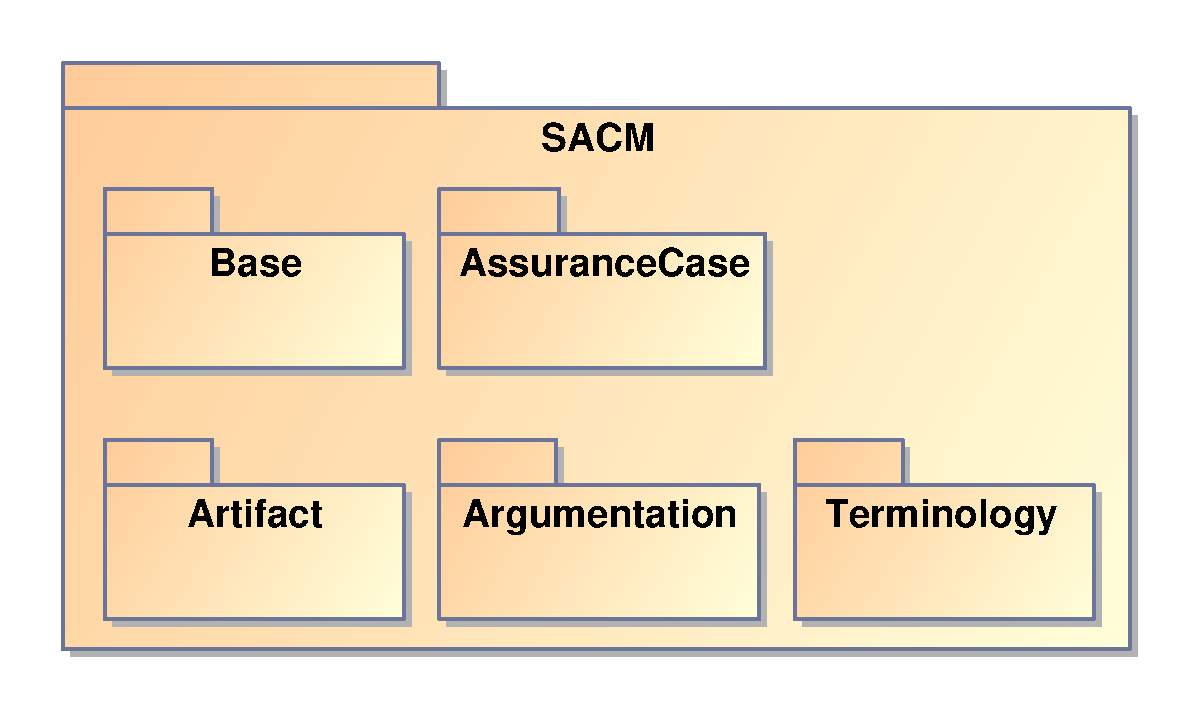
\includegraphics[width=0.6\linewidth]{Overview.eps}
	\caption{Packages of SACM}
	\label{fig:overview}
\end{figure}

\subsection{SACM AssuranceCase Package}
\label{sec:acPack}
Although the \textit{Base} package provides the foundation of SACM, it is necessary to discuss the \textit{AssuranceCase} package first as it provides an insight on how an \textit{Assurance Case} in SACM is organised. The structure of the \textit{AssuranceCase} package is shown in Figure~\ref{fig:ac}.

\begin{figure}
	\centering
	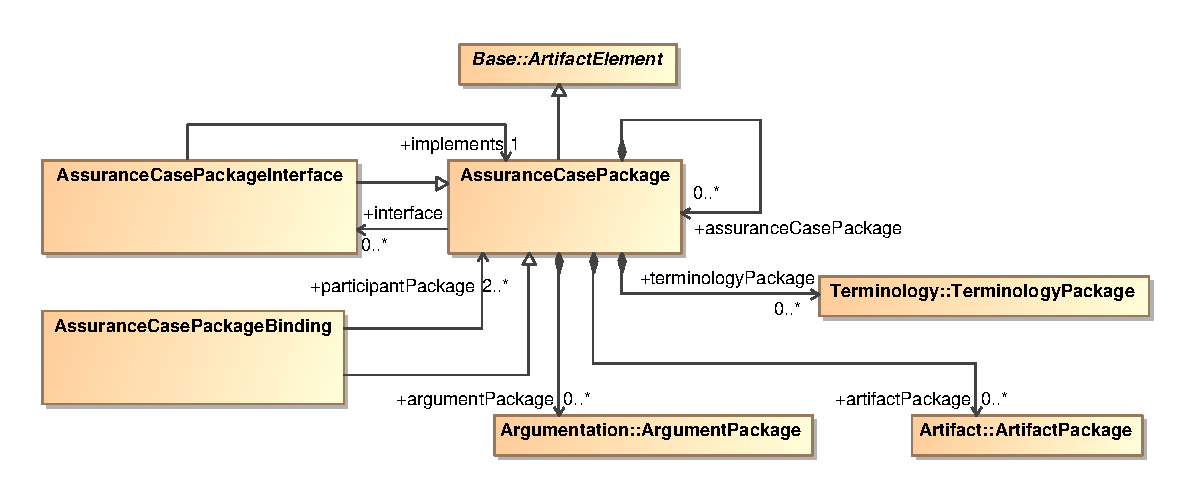
\includegraphics[width=1\linewidth]{AssuranceCase.eps}
	\caption{Packages of SACM}
	\label{fig:ac}
\end{figure}

The core element in the \textit{AssuranceCase} package is the \textit{AssuranceCasePackage} element, which extends the \textit{ArtifactElement} in the \textit{Base} package. The implication is that an \textit{AssuranceCasePackage} can be considered to be an artefact. An \textit{AssuranceCasePackage} can hold a number of \textit{ArgumentPackage}s, \textit{TerminologyPackage}s and \textit{ArtifactPackage}s, which are modeled in the \textit{Argumentation}, \textit{Terminology} and \textit{Artifact} packages respectively.

Sometimes, the developer of an \textit{AssuranceCasePackage} may want to make part of the \textit{AssuranceCasePackage} public so that they can be re-used. Consider the scenario where a system is composed of components A and B and \textit{AsssuranceCasePackage}s ACPA and ACPB are created respectively for A and B (which contain structured argumentations with regard to safety and/or security properties for A and B). The developer may want to make parts of the argumentations public so that during system integration, where A and B are integrated to form a system, their assurance cases ACPA and ACPB can also be integrated to form a new \textit{AssuranceCasePackage}. To disclose only necessary contents externally, one may make use of the \textit{AssuranceCasePackageInterface} to do so. 

It is an usual activity, in the system integration process to integrate assurance cases of systems to form an overall assurance case. SACM handles this scenario with the \textit{AssuranceCasePackageBinding}, which binds two or more \textit{AssuranceCasePackageInterface}s together to form an overall \textit{AssuranceCasePackage}. This particular scenario is discussed in Section~\ref{} \will{example}.

\begin{figure}
	\centering
	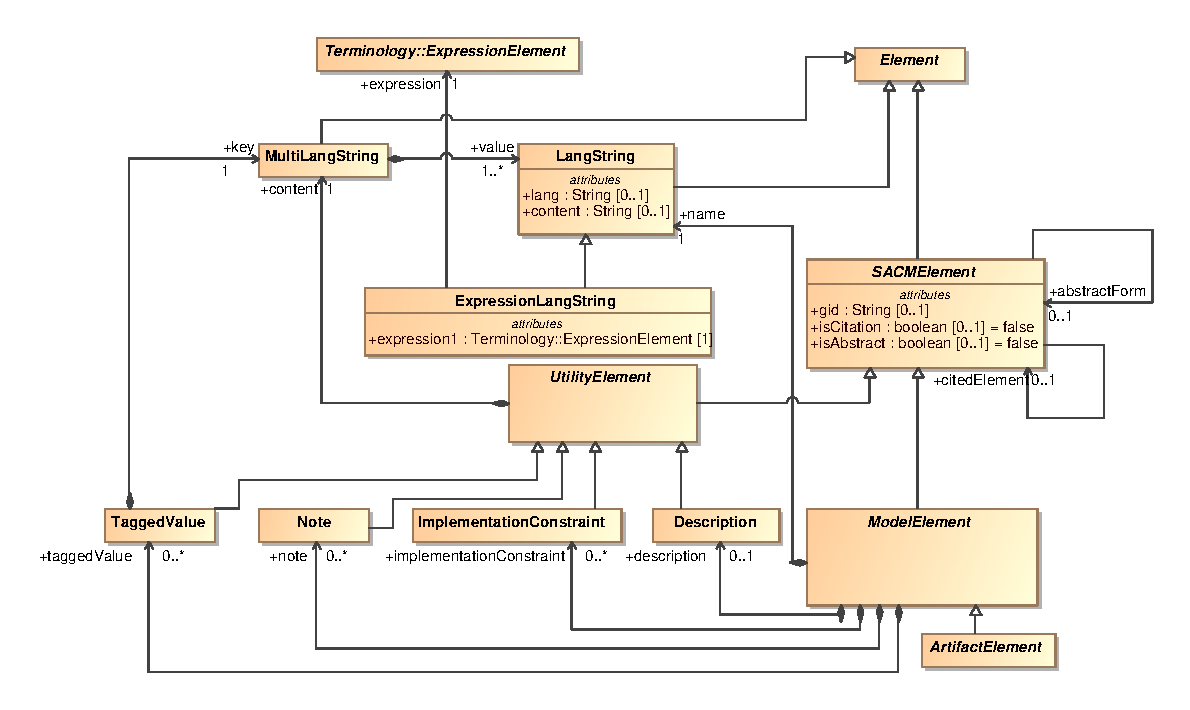
\includegraphics[width=1\linewidth]{Base.eps}
	\caption{Packages of SACM}
	\label{fig:base}
\end{figure}


\subsection{SACM Base Package}
\label{sec:basePack}
The \textit{Base} package captures the foundational concepts of SACM, the structure of the \textit{Base} package is shown in Figure~\ref{fig:base}. The base element of all SACM elements is \textit{Element}. Its direct children are \textit{LangString}, \textit{MultiLangString} and \textit{SACMElement}.

\textit{LangString} is used as an equivalence to \textit{String} (the value of which is held in the \textit{+content} feature), except it captures an additional feature \textit{+lang} which allows the users to define what language is used in the \textit{LangString}. \textit{ExpressionLangString} is used to not only record a \textit{String} in SACM, but also refer to its corresponding \textit{Expression} organised in a \textit{TerminologyPackage}. The usage of \textit{ExpressionLangString} is discussed in Section~\ref{sec:termPack} \textit{MultiLangString}, as its name suggests, is used to express the same semantics using different languages. For example, to express 'hazard' in both English and German, the user can create a \textit{MultiLangString} with two \textit{LangString}, like shown in Figure~\ref{fig:mulitiLang}.

The \textit{MultiLangString} can then be associated to other SACM elements to denote the same meaning. What is more important than multiple natural language support is the support for computer languages. We envision that in the future, system assurance can benefit from automation, so that system assurance can be partially automated. In this case, \textit{MultiLangString} can be used to hold both natural languages and computer languages (e.g. formal languages) to support automated reasoning of argumentations. 

\begin{figure}
	\centering
	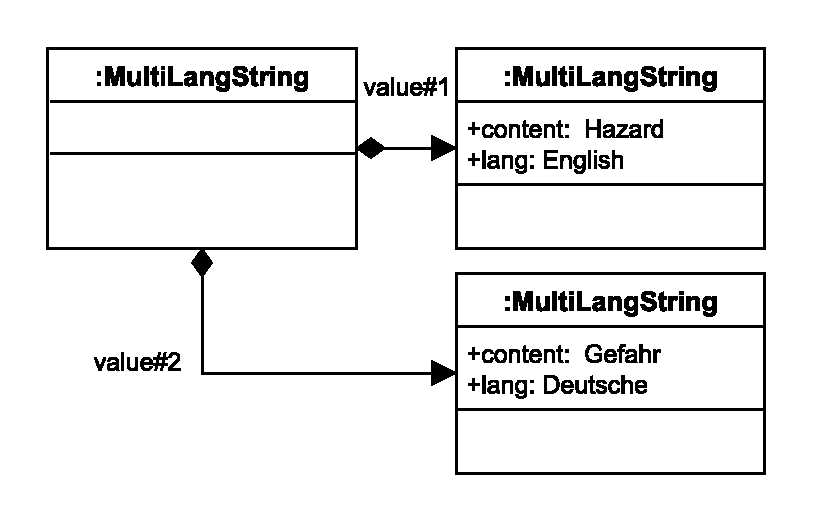
\includegraphics[width=0.5\linewidth]{MultiLangString.eps}
	\caption{Packages of SACM}
	\label{fig:mulitiLang}
\end{figure}

\textit{SACMElement} is an abstract element which lays the foundation of all SACM elements. \textit{SACMElement} can record a \textit{+gid} (\textit{global identification}). 
This means that within the same \textit{AssuranceCasePackage}, each \textit{SACMElement} should have an unique ID. 
\textit{SACMElement} is also able to refer to (or 'cite') other \textit{SACMElement}s, which is useful for implicit references discussed in Section \ref{}\will{example}. The \textit{citedElement} and \textit{isCitation} properties are used for this purpose. A \textit{SACMElement} can also be abstract, denoted by the \textit{isAbstract} property. A \textit{SACMElement} can also be an \textit{abstractForm} of another, which is discussed in Section \ref{}\will{example}. 

\textit{ModelElement} further refines \textit{SACMElement} which contains a \textit{name} (of type \textit{LangString}) and a set of \textit{UtilityElement}s. A \textit{ModelElement} can contain a \textit{Description} which describes its contents. Like previously mentioned, a \textit{Description} can be expressed in any language via its usage of \textit{MultiLangString}. A \textit{ModelElement} can also contain an \textit{ImplementationConstraint}, in some cases, validation rules and/or queries to models are needed for specific \textit{ModelElement}s, \textit{ImplementationConstraint} can be used to specify such constraints in computer languages (e.g. Object Constraint Language~\cite{})\footnote{See Section~\ref{sec:artiPack} for an example.}. A \textit{ModelElement} can also contain a number of \textit{Note}s, to hold additional information rather than descriptions. Finally, a \textit{ModelElement} can also contain a number of \textit{TaggedValue}s, which are essentially \{key, value\} pairs. \textit{TaggedValue} can be considered as an extension mechanism to allow the users to associate additional features to a \textit{ModelElement} (other than the features modelled in the current version of SACM).

The \textit{Base} package also defines the \textit{ArtifactElement}, in the sense that all elements that extend \textit{ArtifactElement} are considered to be \textit{Artifact}s. The reason for this is discussed in Section~\ref{}\will{example}. 

In summary, the \textit{Base} package lays the foundation for SACM, it provides facilities not to only express assurance cases (to be precise, assurance case models) in natural language, but also in computer languages. The \textit{Base} package also provides a number of \textit{UtilityElement}s so that the user can use them to describe \textit{ModelElement}s as precisely as possible.

\begin{figure}
	\centering
	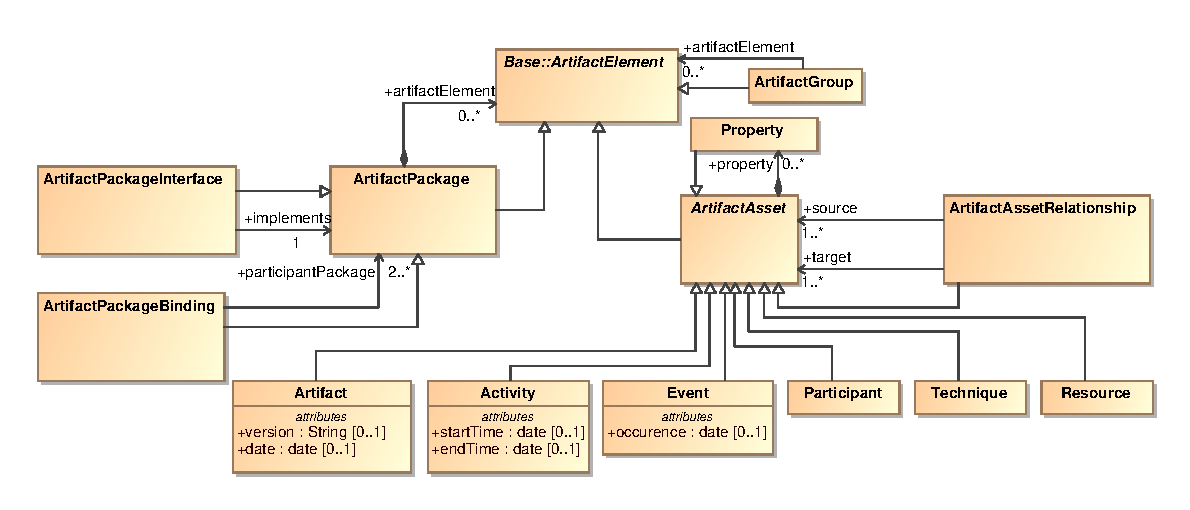
\includegraphics[width=1\linewidth]{Artifact.eps}
	\caption{Packages of SACM}
	\label{fig:arti}
\end{figure}

\subsection{SACM Artifact Package}
\label{sec:artiPack}
Before delving into the \textit{Argumentation} package, it is necessary to discuss the \textit{Artifact} package. The structure of the \textit{Artifact} package is shown in Figure~\ref{fig:arti}. 
All elements in the \textit{Artifact} package extend \textit{ArtifactElement} in the \textit{Base} package. \textit{ArtifactElement}s are organised in \textit{ArtifactPackage}s to promote modularity. SACM considers integration of assurance cases at the level of \textit{ArtifactPackage}, \textit{ArtifactPackageInterface} and \textit{ArtifactPackageBinding} are used for this purpose.

\textit{ArtifactGroup} is a new concept introduced in SACM 2.0. As \textit{ArtifactPackage} can contain rather a large number of \textit{ArtifactElement}s, the \textit{ArtifactGroup} provides the user with a means to selectively group \textit{ArtifactElement}s, so that the user can group/view \textit{ArtifactElement}s with their defined criteria.

\textit{ArtifactAsset} allows the users to create corresponding artefact elements in SACM, it can contain a number of \textit{Property}-ies to hold user-defined properties. \textit{Artifact} is used to record a piece of information (such as hazard log, failure logic models, etc). \textit{Activity} is used to record an activity (e.g. specification of requirements). \textit{Event} is used to record an event (e.g. creation/modification of \textit{Artifact}s). \textit{Participant} is used to record participants involved in \textit{ArtifactAsset}s. \textit{Technique} is used to record the techniques used in \textit{Activities}. \textit{Resource} is used to record a piece of resource, usually in the form of some electronic file. And finally, \textit{ArtifactAssetRelationship} is used to link \textit{ArtifactAsset}s (e.g. connecting \textit{Activity} to \textit{Participant}s). Note that the \textit{ArtifactAssetRelationship} is a generic relationship, however, the user can choose to use \textit{Property} to specify the purpose of an \textit{ArtifactAssetRelationship}. 

\begin{figure}
	\centering
	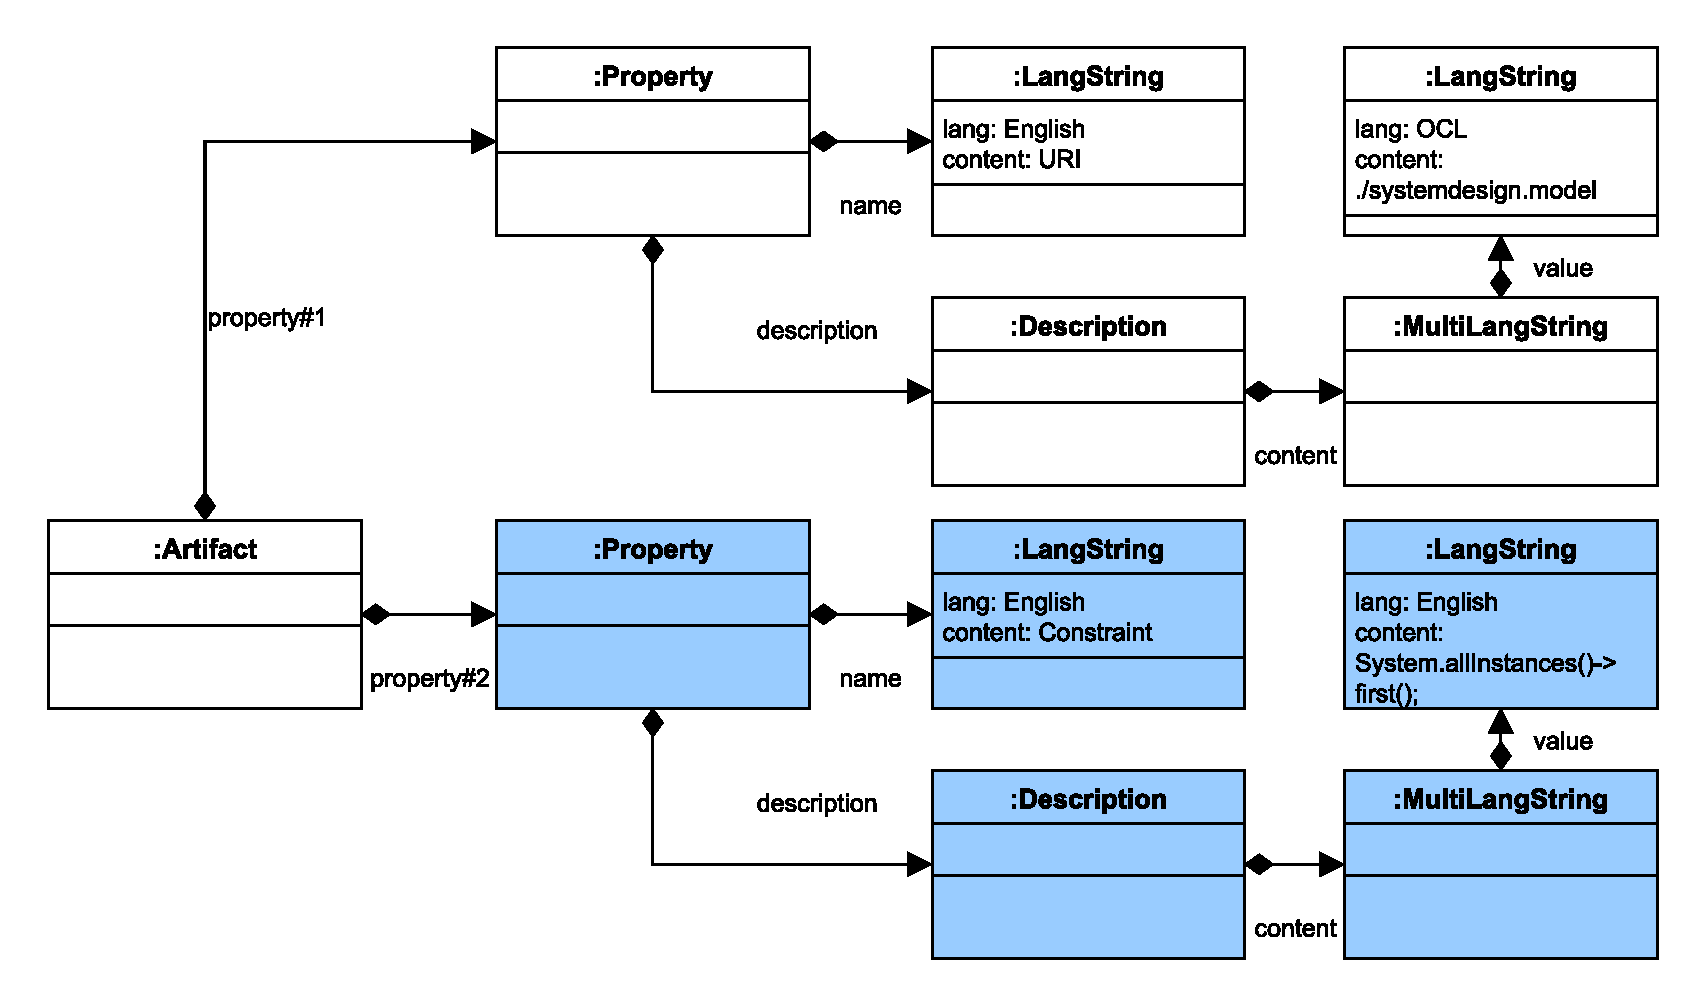
\includegraphics[width=1\linewidth]{artifact2.eps}
	\caption{External reference using \textit{Property}.}
	\label{fig:artifact1}
\end{figure}

One open question regarding the \textit{Artifact} package is how to refer to external materials (such as system requirement, system design model, system failure logic model, etc.). To achieve automation, it is necessary to have a means to refer to external materials (especially models) so that all information can be gathered together to form an assurance case. 
The user may make use of the \textit{Property} element, as shown in Figure~\ref{fig:artifact1} (consider elements filled in \textit{white} first).

In Figure~\ref{fig:artifact1} where elements are filled in \textit{white}, a \textit{Property} is associated to an \textit{Artifact}\footnote{The \textit{Artifact} should have its own features such as name and description, which is omitted here.}, which has a \textit{name} (of type \textit{LangString}): 'URI' and a \textit{Description}, which in turn specifies a file on local folder (systemdesign.model). In this way, the \textit{Property} element is used as a reference to a local file. 

There are often cases that the user may want to refer to a single element (or a collection of elements) in a model. If this is the case, an additional \textit{Property} can be used, as shown in Figure~\ref{fig:artifact1} (elements filled in \textit{white}). 
For the \textit{Property}, its name is \textit{Constraint} and \textit{OCL} is used in its description. In this example, two \textit{Properties} should be used together (first using \textit{URI} to locate the model, then using \textit{Constraint} to query the model).

SACM does not restrict how external materials should be referenced, the description provided above is one way of achieving it. It also depends on tool implementations on how external references should be handled. 
\begin{figure}[ht!]
	\centering
	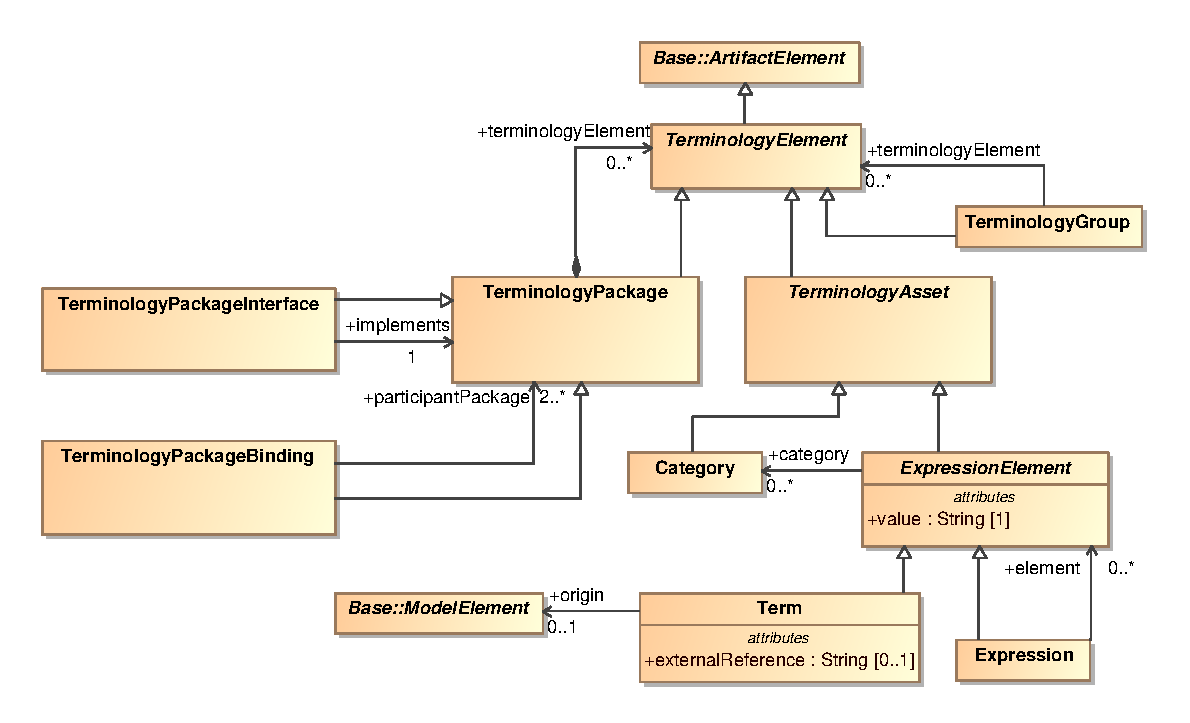
\includegraphics[width=1\linewidth]{Terminology.eps}
	\caption{Packages of SACM}
	\label{fig:term}
\end{figure}
\subsection{SACM Terminology Package}
\label{sec:termPack}
The \textit{Terminology} package captures concepts that enable the users of SACM to describe their argumentations in greater precision. The structure of the \textit{Terminology} package is shown in Figure~\ref{fig:term}.

The root element of the \textit{Terminology} package is \textit{TerminologyElement} which also extends \textit{ArtifactElement} in the \textit{Base} package. \textit{TerminologyGroup}, \textit{TerminologyAsset} and \textit{TerminologyPackge} are direct children of \textit{TerminologyElement}. \textit{TerminologyAsset}s are organised in \textit{TerminologyPackage}s to promote modularity. SACM considers integration of assurance cases at the level of \textit{TerminologyPackage}. \textit{TerminologyInterface} and \textit{TerminologyPackageBinding} are used for this purpose.

As \textit{TerminologyPackage} can also get large in size, \textit{TerminologyGroup} provides the user with a means to selectively group \textit{TerminologyAsset}s, so that the user of SACM can group/view \textit{TerminologAsset}s as they wish.

\begin{figure}
	\centering
	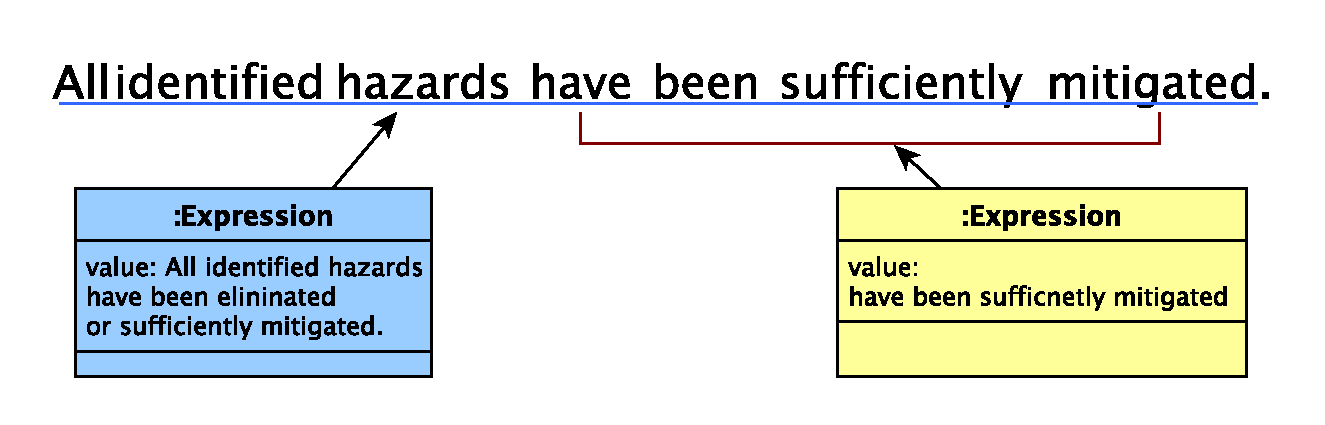
\includegraphics[width=1\linewidth]{expression.eps}
	\caption{Example use of \textit{Expression}.}
	\label{fig:expression}
\end{figure}

\textit{ExpressionElement} captures the concept of different kinds of expressions used in argumentations. \textit{ExpressionElement} holds a \textit{value} (of type String). \textit{ExpressionElement} can either be an \textit{Expression} or a \textit{Term}. An \textit{Expression} is used to model phrases and sentences. For example, when stating a sentence: \textbf{All identified hazards have been sufficiently mitigated.}, the \textit{Expression} element can be used to to capture this sentence as shown in Figure~\ref{fig:expression} (element filled with cyan colour). Alternatively, the users of SACM may choose to capture each word in the sentence as an \textit{Expression}, as shown in Figure~\ref{fig:expression} (element filled with white colour). The idea behind \textit{Expression} is to store words/phrases/sentences in the \textit{TerminologyPackage} like a dictionary, so that the \textit{Expression}s can be re-used. Of course the example in Figure~\textit{fig:expression} does not add too much value to the assurance case, in realistic scenarios, only phrases that can be re-used should be captured in \textit{Expression}s. This is completely up to the user and tool developers of SACM. 

\begin{figure}
	\centering
	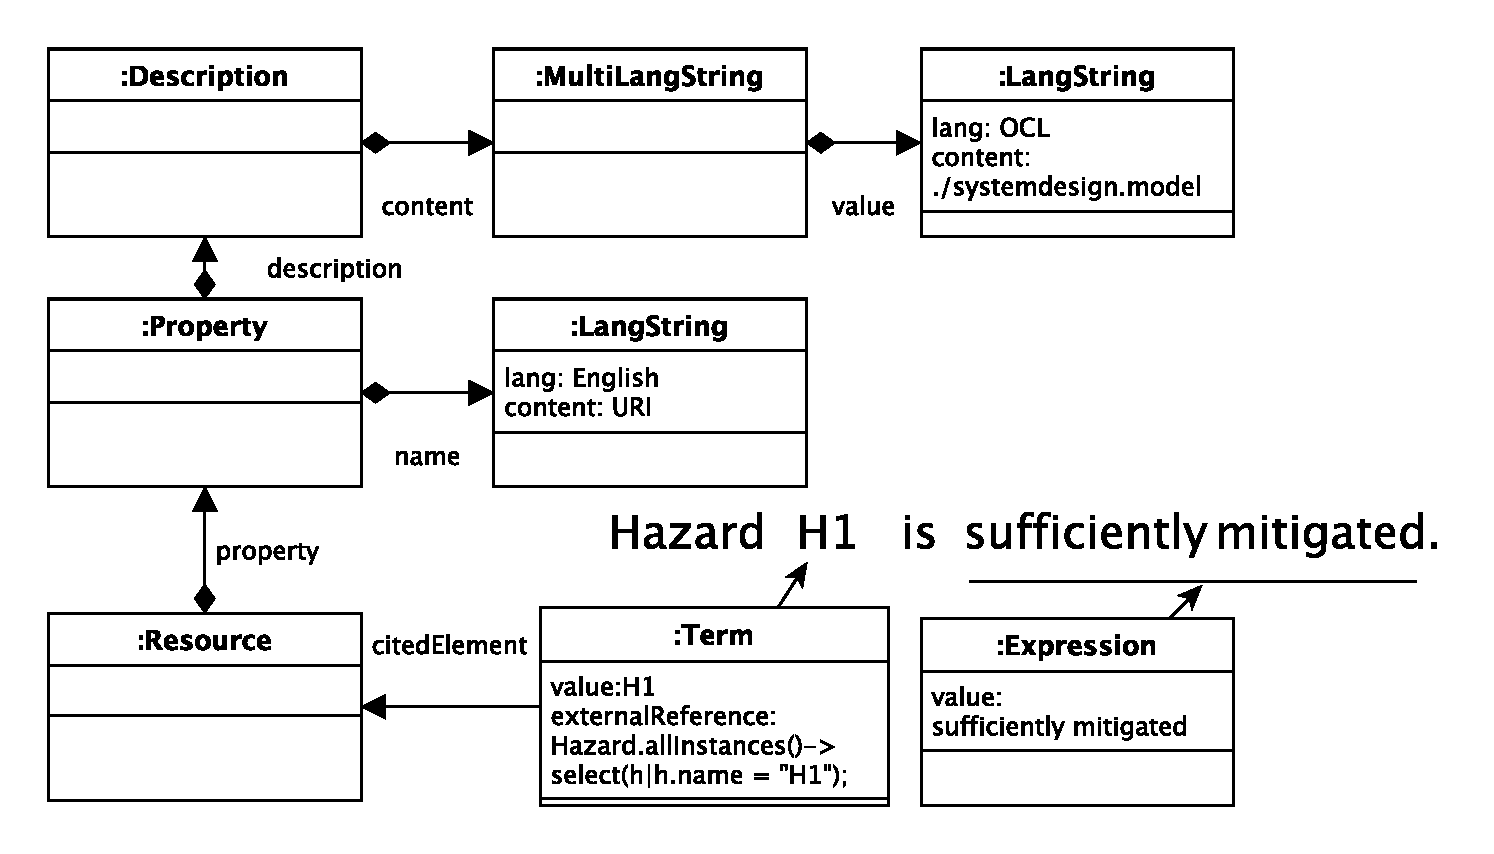
\includegraphics[width=1\linewidth]{term.eps}
	\caption{Example use of \textit{Expression} and \textit{Term}.}
	\label{fig:termExample}
\end{figure}

The \textit{Term} element is used to capture a terminology used in the process of system assurance. For example, in Figure~\ref{fig:termExample} (first consider elements filled in white), a statement is made: \textbf{Hazard \textit{H1} is sufficiently mitigated.} Within the sentence, \textit{H1} in fact may cross-references to an identified hazard in a hazard log. Thus, \textit{H1} can be captured using a \textit{Term}. 
The location of the hazard log can be captured using a \textit{Resource}\footnote{The details of the \textit{Resource} is omitted.} in the \textit{Artifact} package, where the location of the \textit{Resource} is captured using \textit{Property}. 
In order to point to a specific model element (in this case, model element H1 in the hazardLog.model), the user may use OCL in the +externalReference feature of the \textit{Term}. This is illustrated in Figure~\ref{fig:termExample}.
Again, SACM does not restrict how external references should be handled, the description provided above is one way of achieving it. It also depends on tool implementations on how external references are handled. 

Sometimes, a term may refer to a \textit{ModelElement} within the assurance case (via the +origin feature), we will discuss this in Section~\ref{}.\will{example}

The users of SACM may also organise \textit{ExpressionElement} into \textit{Categories}. For example, the users may create an \textit{Category} of Hazard, and associate the \textit{Term} H1 to it. 
\subsection{SACM Argumentation Package}
\label{sec:argPack}
\begin{figure}
	\centering
	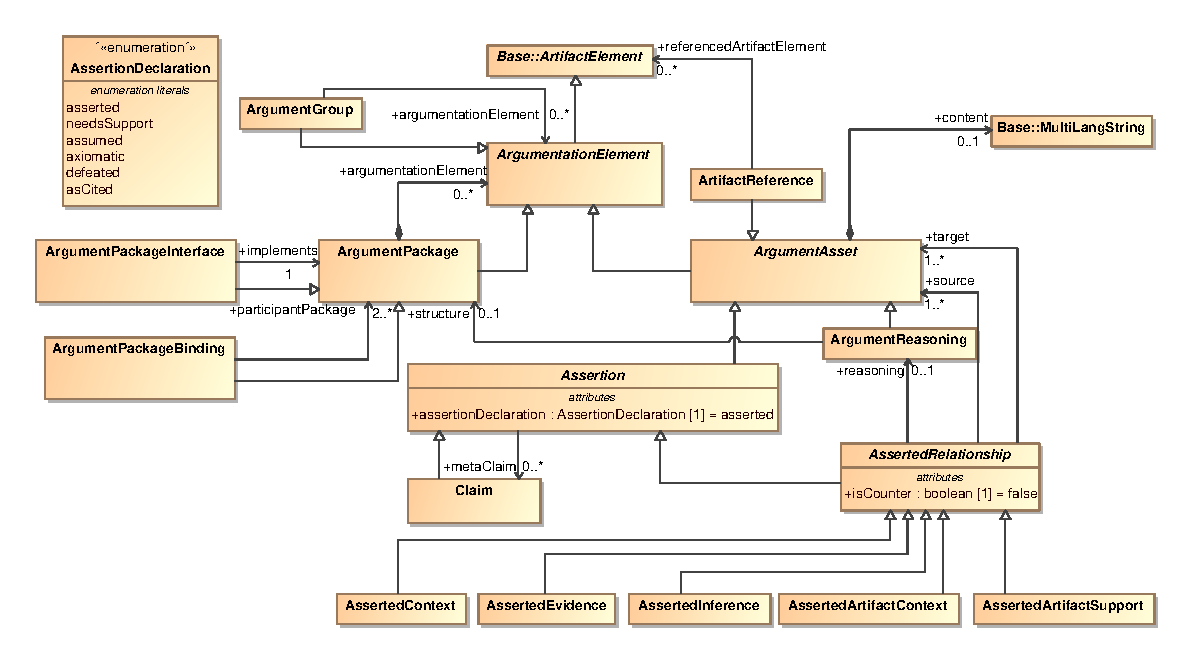
\includegraphics[width=1\linewidth]{Argumentation.eps}
	\caption{Packages of SACM}
	\label{fig:arg}
\end{figure}
The \textit{Argumentation} Package captures the concepts required to model structured arguments regarding system properties. The structure of the \textit{Argumentation} package is shown in Figure~\ref{fig:arg}.
The root element of the \textit{Argumentation} package is the \textit{ArgumentationElement}, which is a direct child of \textit{ArtifactElement} in the \textit{Base} package. This implies that all elements in the \textit{Argumentation} package are also considered to be artifacts. 

To promote modularity, argumentations are organised in \textit{ArgumentPackage}s. \textit{ArgumentationPackage} can contain a number of \textit{ArgumentationElement}, which can either be \textit{ArgumentPackage}s (and their children) or \textit{ArgumentAsset}s. \textit{ArgumentAsset} can store a \textit{content}, as discussed in Section~\ref{sec:basePack}, the content can be in any language\footnote{Via the usage of \textit{MultiLangString}}.

\textit{ArgumentAsset} and its children are the elements that form the structured argumentation in the \textit{Argumentation} package. An \textit{Assertion} has an \textit{AssertionDeclaration} to distinguish different kinds of \textit{Assertion}s. The \textit{AssertionDeclaration}s are as follows: 

\begin{itemize}
	\item \textbf{asserted} - the default declaration, means that the \textit{Assertion} is given and is supported by evidence;
	\item \textbf{needsSupport} - a flag indicating that the \textit{Assertion} is not supported yet (needs further development);
	\item \textbf{assumed} - a flag indicating that the truth of the \textit{Assertion} is assumed although no supporting evidence is provided;
	\item \textbf{axiomatic} - a flag indicating that the truth of the \textit{Assertion} is axiomatically true without further supporting evidence;
	\item \textbf{defeated} - a flag indicating that the truth of the \textit{Assertion} is invalidated by a counter-evidence and/or argumentation;
	\item \textbf{asCited} - when an \textit{Assertion} 'cite's another \textit{Assertion} (via the +citedElement property in \textit{SACMElement}), the truth of the \textit{Assertion} is transitively derived from the value of the cited \textit{Assertion}.
\end{itemize}

The use of \textit{AssertionDeclaration} will be illustrated in Section~\ref{sec:claims}.
Sometimes it is necessary to argue the confidence in the arguments provided in the assurance case. This can be achieved using the \textit{+metaClaim} feature of the \textit{Assertion} element. \textit{+metaClaim} is discussed in Section~\ref{}. \will{example}

\textit{Claim} and \textit{AssertedRelationship} are the core elements of the \textit{Argumentation} package. \textit{AssertedRelationship} are used to connect \textit{ArgumentAsset}s to form structured argumentation (\textit{AssertedRelationship}s can also be \textit{counter} relationships, indicated by the \textit{+isCounter} feature):

\begin{itemize}
	\item \textbf{AssertedCotnext} - this relationship is used to connect contextual \textit{Claim}s to \textit{asserted} \textit{Claim}s;
	\item \textbf{AssertedEvidence} - this relationship is used to connect evidence (referenced via \textit{ArtifactReference}) to \textit{Claim}s;
	\item \textbf{AssertedInference} - this relationship is used to connect \textit{asserted} \textit{Claim}s to an \textit{asserted} \textit{Claim};
	\item \textbf{AssertedArtefactContext} - this relationship is used to connect contextual artefacts (via \textit{ArtifactReference}) to an artefact (via \textit{ArtifactReference});
	\item \textbf{AssertedArtefactSupport} - this relationship is used to connect evidential artefacts (via \textit{ArtifactReference}) to an artefact (via \textit{ArtifactReference}).
\end{itemize}

\textit{ArtifactReference} is a type of \textit{ArgumentAsset}, which is able to refer to an \textit{ArtifactElement}. \textit{ArtifactReference} is typically used to refer to evidence stored in an \textit{Artifact} package. In addition, it can refer to any element that extend \textit{ArtifactElement} (all elements in the \textit{AssuranceCase}, \textit{Argumentation}, \textit{Artifact} and \textit{Terminology} packages are \textit{ArtifactElement}s).

\textit{ArgumentReasoning} is also a type of \textit{ArgumentAsset}, it is used to provide a explanatory description for an \textit{AssertedRelationship}. An detailed discussion of \textit{ArgumentReasoning} is in Section~\ref{}. \will{example}

\textit{Claim}s, \textit{AssertedRelationship}s, \textit{ArtifactReference} and \textit{ArgumentReasoning} form a structured argumentation network, which are stored in \textit{ArgumentPackage}s. 

\subsection{Summary}
In this section, we discussed the packages defined in SACM. We explain the intended semantics of the elements in the packages and we used some in-place examples to illustrate how SACM can be used to construct a system assurance case with argumentations regarding system properties (i.e. safety and/or security) and its supporting evidence/artefact (using the \textit{Artifact} and \textit{Terminology} packages of SACM). In the next section, we will illustrate how SACM can be used with more concrete examples.

\section{SACM: Examples}
In this section, we provide concrete examples on how SACM is used to construct structured argumentation, and how SACM can be used to form argumentation patterns (similar to GSN argument patterns). 

\subsection{Example: Assertion Declarations}
\label{sec:claims}

\begin{figure}
	\centering
	\begin{minipage}[b]{0.7\textwidth}
		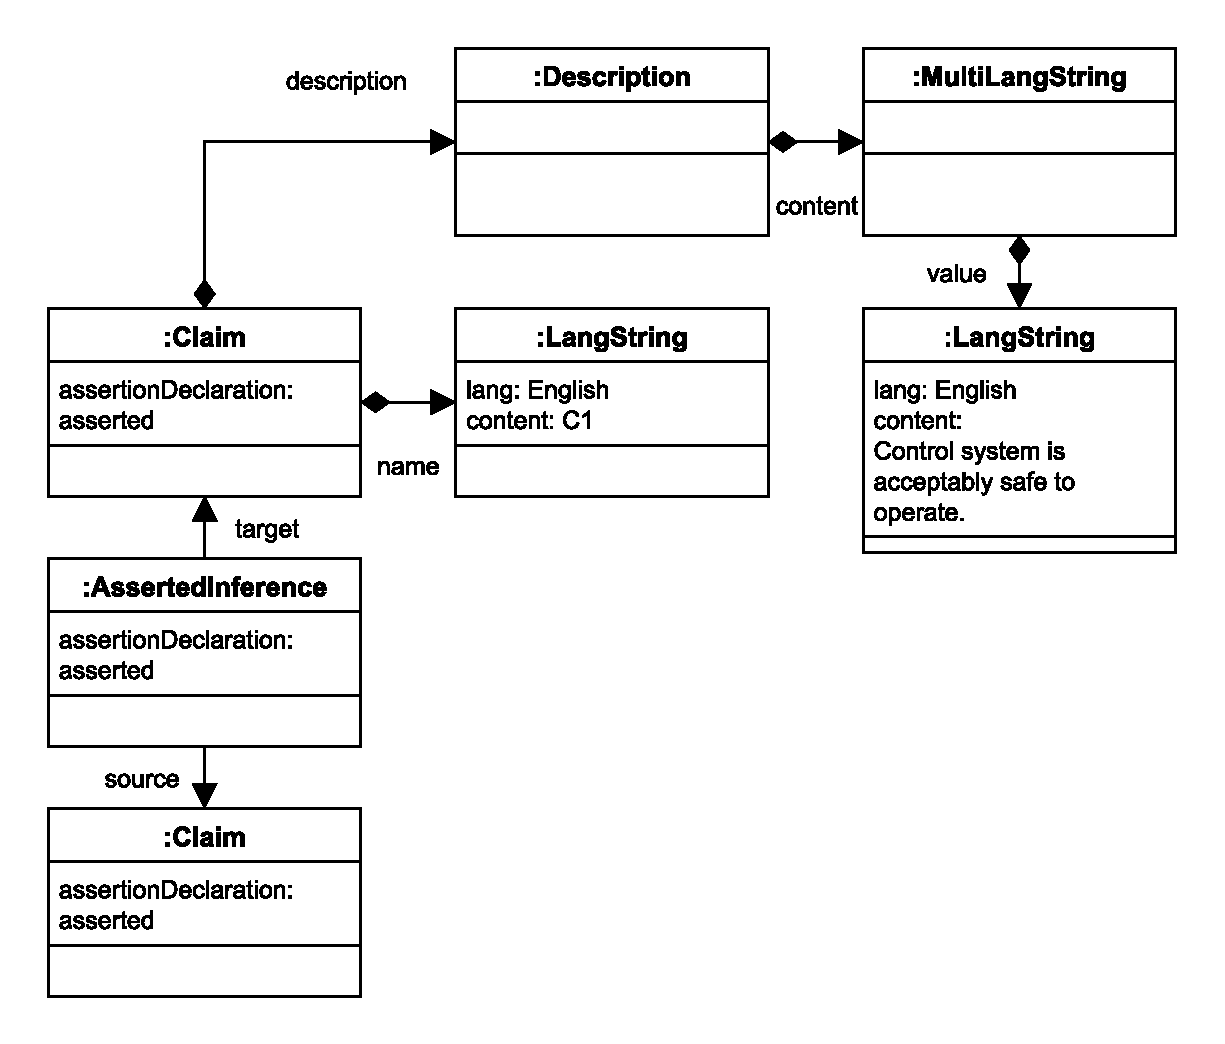
\includegraphics[width=\textwidth]{assertedClaim.eps}
		\caption{An \textbf{asserted} \textit{Claim} in SACM.}
		\label{fig:assertedClaim}
	\end{minipage}
	\hfill
	\begin{minipage}[b]{0.28\textwidth}
		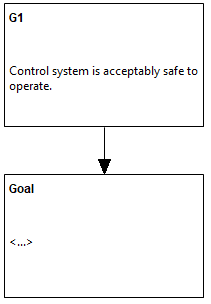
\includegraphics[width=\textwidth]{goal_asserted.png}
		\caption{A \textit{Goal} in GSN.}
		\label{fig:goalingsn}
	\end{minipage}
\end{figure}

Figure~\ref{fig:assertedClaim} provides an example on how to construct a \textit{Claim}. A \textit{Claim} can have a name and a description, captured by \textit{LangString} and \textit{Description} respectively. A \textit{Claim} is \textbf{asserted} if it is supported by other \textit{Claim}s. In this example, it is connected by an \textit{AssertedInference} with another \textit{Claim} (details ommitted). The equivalence of \textit{Claim} C1 in Figure~\ref{fig:assertedClaim} in GSN is provided in Figure~\ref{fig:goalingsn}, where the \textit{Goal} G1 bears the same semantics with C1 (and how \textit{Goal} G1 is supported by subsequent \textit{Goal}s\footnote{Details of \textit{Goal}s are omitted.}).

\begin{figure}
	\centering
	\begin{minipage}[b]{0.7\textwidth}
		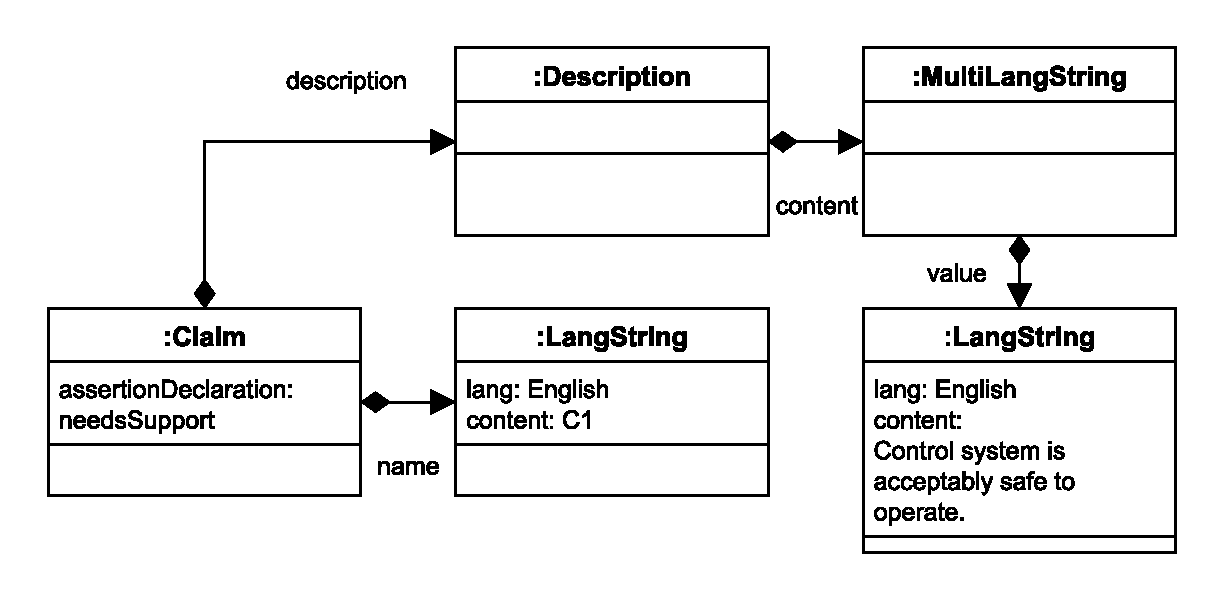
\includegraphics[width=\textwidth]{needsSupportClaim.eps}
		\caption{A \textbf{needsSupport} \textit{Claim} in SACM.}
		\label{fig:needsSupportClaim}
	\end{minipage}
	\hfill
	\begin{minipage}[b]{0.28\textwidth}
		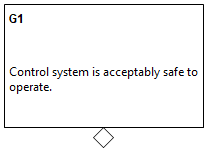
\includegraphics[width=\textwidth]{undevGoal.png}
		\caption{A \textit{Goal} in GSN.}
		\label{fig:undevGoal}
	\end{minipage}
\end{figure}

Like previously mentioned, a \textit{Claim} can be marked as \textbf{needsSupport}. Figure~\ref{fig:needsSupportClaim} illustrates the use of this declaration. A \textit{Claim} that is not supported by any argument/evidence should be marked as \textbf{needsSupport}. The equivalence of this \textit{Claim} is shown in Figure~\ref{fig:undevGoal}, where \textit{Goal} G1 bears the same semantics of \textit{Claim} C1. When a \textit{Goal} is not supported by argument/evidence, it is be marked as \textit{undeveloped}. 

\begin{figure}
	\centering
	\begin{minipage}[b]{0.7\textwidth}
		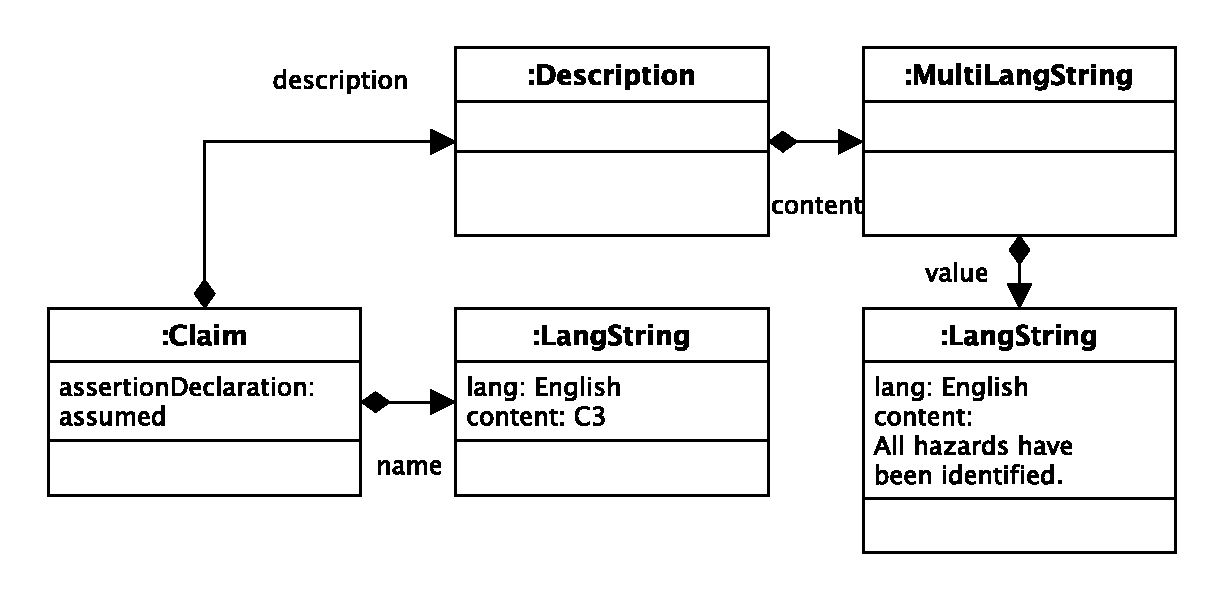
\includegraphics[width=\textwidth]{assumedClaim.eps}
		\caption{A \textbf{assumed} \textit{Claim} in SACM.}
		\label{fig:assumedClaim}
	\end{minipage}
	\hfill
	\begin{minipage}[b]{0.28\textwidth}
		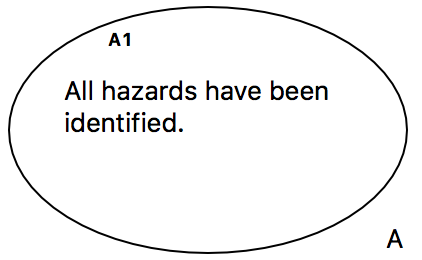
\includegraphics[width=\textwidth]{example_assumption.png}
		\caption{An \textit{Assumption} in GSN.}
		\label{fig:example_assumption}
	\end{minipage}
\end{figure}

A \textit{Claim} marked as \textbf{assumed} is used to state an assumption in the argumentation. Figure~\ref{fig:assumedClaim} illustrates an \textbf{assumed} \textit{Claim} in SACM (where the user assumes that \textit{all hazards have been identified}). The users are responsible to declare that a \textit{Claim} is \textbf{assumed} when they make assumptions about the system. The equivalence for \textbf{assumed} \textit{Claim} is an \textit{Assumption} in GSN, as shown in Figure~\ref{fig:example_assumption}.

\begin{figure}
	\centering
	\begin{minipage}[b]{0.7\textwidth}
		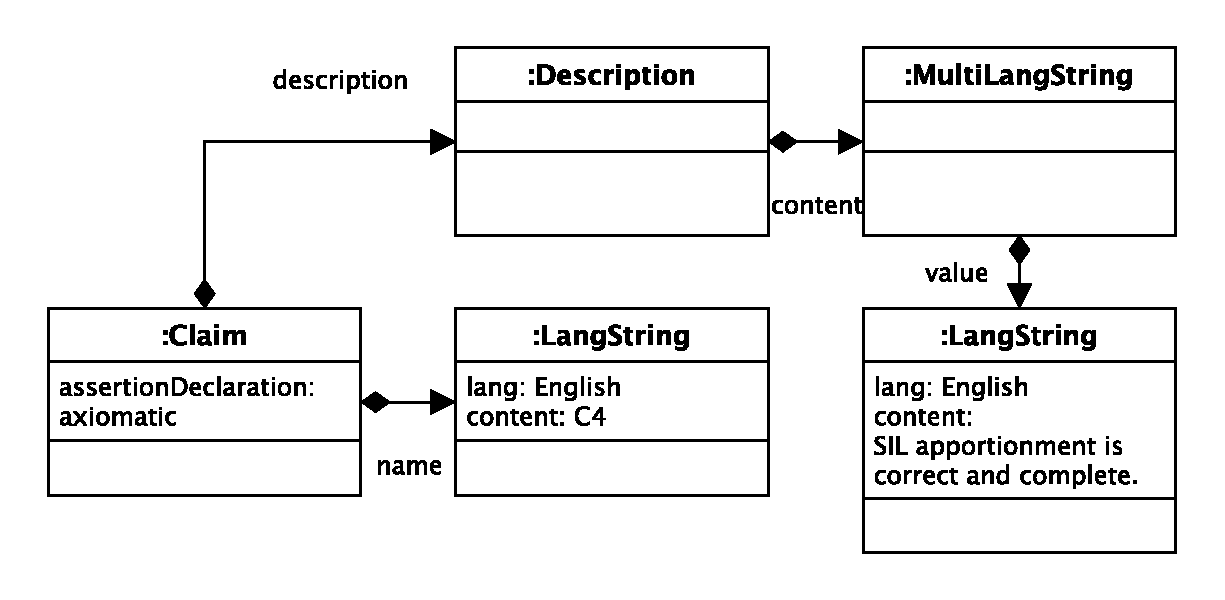
\includegraphics[width=\textwidth]{axiomaticClaim.eps}
		\caption{A \textbf{axiomatic} \textit{Claim} in SACM.}
		\label{fig:axiomaticClaim}
	\end{minipage}
	\hfill
	\begin{minipage}[b]{0.28\textwidth}
		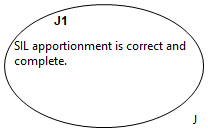
\includegraphics[width=\textwidth]{example_justification.png}
		\caption{A \textit{Justification} in GSN.}
		\label{fig:example_justification}
	\end{minipage}
\end{figure}

A \textit{Claim} marked as \textbf{axiomatic} is used to state a well agreed fact (presumably among stakeholders), which does not need any further support by arguments/evidence. The equivalent of an \textbf{axiomatic} \textit{Claim} in GSN is a \textit{Justification}, which does not need further supporting argument/evidence to support its content. Figure~\ref{fig:axiomaticClaim} and Figure~\ref{fig:example_justification} illustrates the use of \textbf{axiomatic} \textit{Claim} and \textit{Justification} respectively.

\begin{figure}
	\centering
	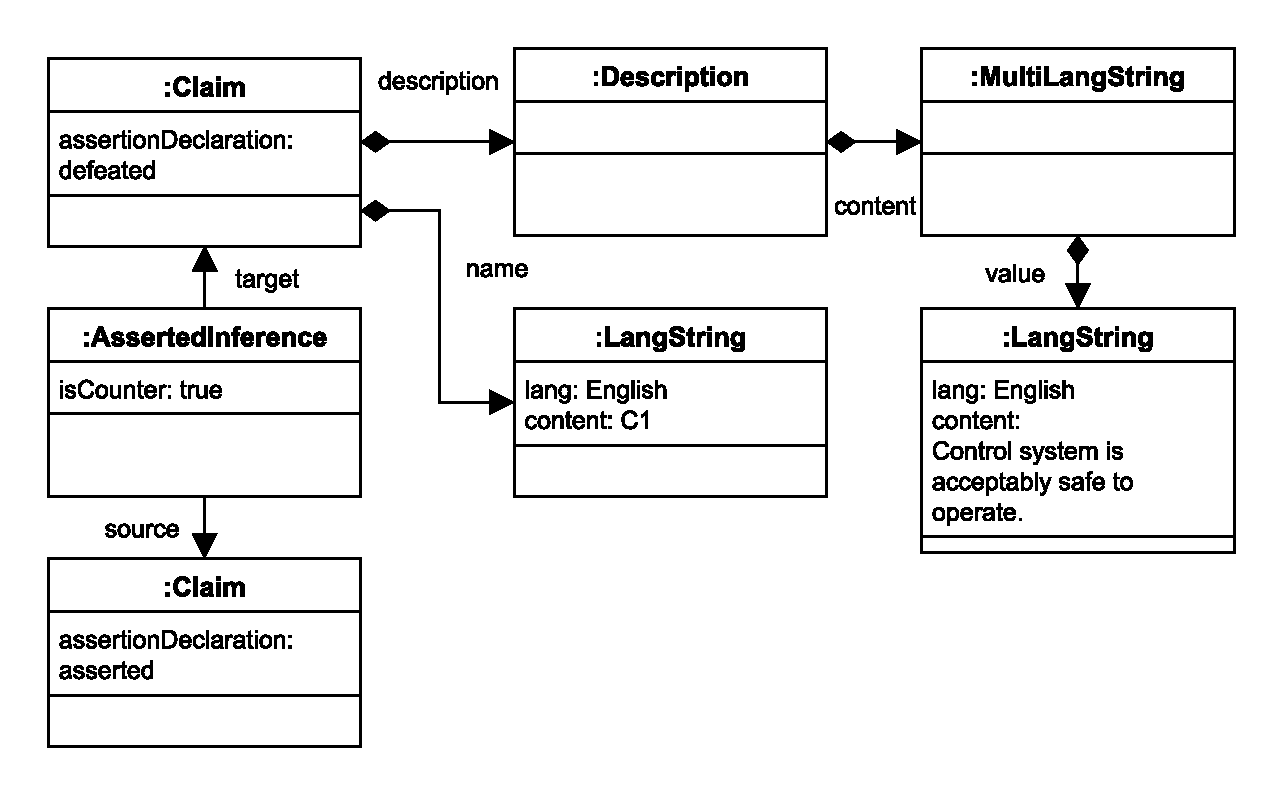
\includegraphics[width=0.8\linewidth]{defeatedClaim.eps}
	\caption{A \textbf{defeated} \textit{Claim}.}
	\label{fig:defeatedClaim}
\end{figure}
A \textit{Claim} is marked as \textit{defeated} if the truth of the claim is proven to be false by supporting argument/evidence. Figure~\ref{fig:defeatedClaim} provides an example of a \textbf{defeated} \textit{Claim}, the \textit{Claim} C1 is connected with another \textit{Claim} (we do not consider the detail of this \textit{Claim} for this example) by an \textit{AssertedInference}, but with its +isCounter feature to be \textit{true}. This means that the \textit{AssertedInference} is a counter-argument, which negates the truth of \textit{Claim} C1 to be \textit{false}.

\begin{figure}
	\centering
	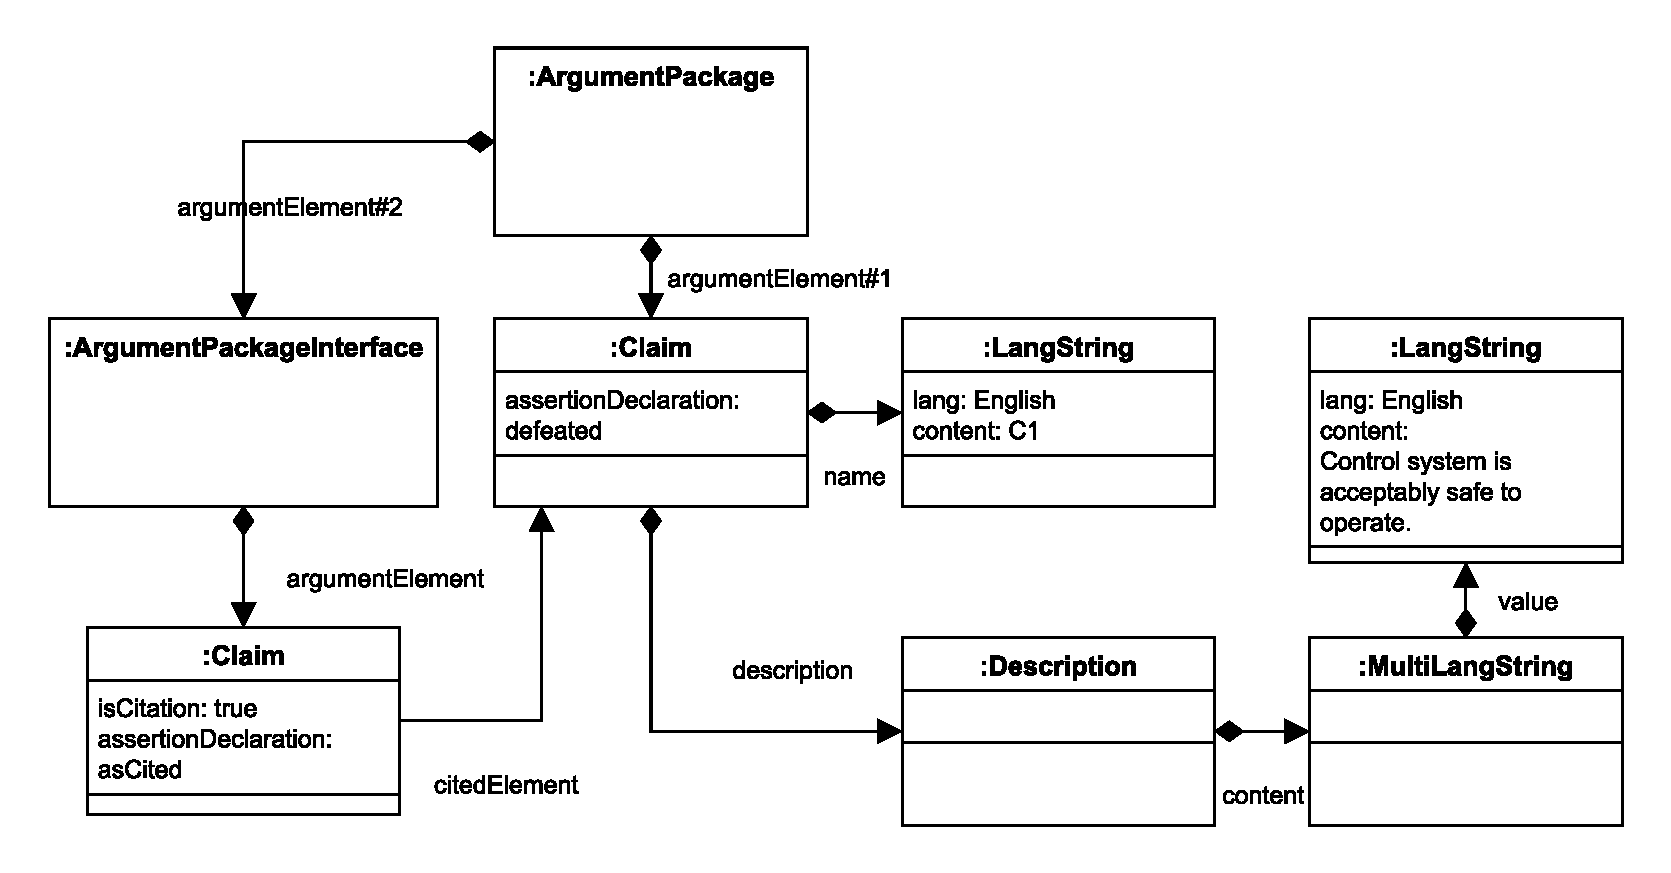
\includegraphics[width=1\linewidth]{asCitedClaim.eps}
	\caption{An \textbf{asCited} \textit{Claim}.}
	\label{fig:asCitedClaim}
\end{figure}

As previously discussed, the users of SACM are able to selectively disclose the content of an \textit{ArgumentPackage} via the use of \textit{ArgumentInterface}. Figure~\ref{fig:asCitedClaim} illustrates how an \textit{ArgumentPackageInterface} can be used. In this example, a \textit{Claim} C1 is held within an \textit{ArgumentPackage}, which contains an \textit{ArgumentPackageInterface} that in turn contains another \textit{Claim}, which is a citation. The \textit{Claim} 'cites' C1 in the \textit{ArgumentPackage} via the \textit{citedElement} feature (which is defined in the \textit{SACMElement} element in the \textit{Base} package). Hence, the \textbf{asCited} declaration on the \textit{Claim} should be used, which means that the truth of the \textit{Claim} as a citation, depends on the \textit{Claim} that it cites (in this case, \textit{Claim} C1).

\subsection{Example: Asserted Relationships}
The intent of \textit{Claim}s are declared using \textit{AssertionDeclaration}s, as previously demonstrated. Different types of \textit{Claim}s are then connected using different \textit{AssertedRelationship}s to form a structured argumentation. 

\subsection{Example: Argumentation Patterns}

\subsection{Example: A case study on the European Train Control Systems (ETCS)}